\subsection{Product description}
\label{sec:product-desc}

% What kind of product
An actual automotive \gls{asic} was tested to highlight a practical case of functional failure.
The tested \gls{asic} performs several high-level and critical functions in the car.

% What kind of failure
The failure was discovered while reducing the amount of external devices, to test the impact on the robustness.
With less external devices, the bill of materials of the electronic system is reduced and the system costs less to manufacture.
It must be clarified that with the normal configuration, the failure never happens (within limits of the \gls{esd} tester).
It can only be reproduced in this lowered configuration.

% Difference of configs
The input used during the tests to inject the \gls{ESD} is the battery supply connection.
The normal configuration uses strong differential and common-mode filtering on this input.
This technique very effectively deviates the stress current into a ground before it even has a chance to reach the tested chip.
In the lowered-configuration, only a reduced differential filtering is present on the input.

% What is being tested
Inside the \gls{ic}, the study focuses on the primary supply function.
More specifically, the behavior of a 2.5V internal DC-DC LDO (glossary ?) regulator is under test.
This function is responsible for waking up all other integrated functions, and powers digital cells.
It plays a key part in the device's operation, and constitutes an interesting study case.
Also, this function requires for normal operation a large stabilisation capacitor that cannot be integrated on silicon.
A pin is exposed externally to let the board manufacturer connect such a capacitor at the board level.
This pin makes for a very easy monitoring point during tests, without needing to open the package to measure signals.

% Global architecture
Fig. \ref{fig:system_architecture} details the architecture of a typical system using the chip under test.

\begin{figure}[!htbp]
  \centering
  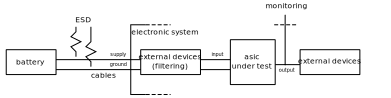
\includegraphics[width=0.9\textwidth]{src/3/figures/architecture_system.pdf}
  \caption{Overview of the system architecture}
  \label{fig:system_architecture}
\end{figure}

GO DOWN INTO ASIC, explain architecture a bit

\begin{figure}[!htbp]
  \centering
  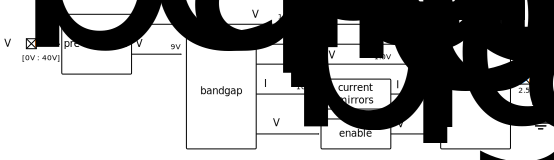
\includegraphics[width=0.9\textwidth]{src/3/figures/monitored_function.pdf}
  \caption{Architecture of the monitored function}
  \label{fig:monitored_function_first}
\end{figure}

SHOW Startup curves ?
